% Contributions are much appreciated, in order to contribute to this project, head over to this repository:
% https://github.com/bshramin/uofa-eng-assignment

\documentclass[11pt,letterpaper]{article}
\textwidth 6.5in
\textheight 9.in
\oddsidemargin 0in
\headheight 0in
\usepackage{graphicx}
\usepackage{fancybox}
\usepackage[utf8]{inputenc}
\usepackage{epsfig,graphicx}
\usepackage{multicol,pst-plot}
\usepackage{pstricks}
\usepackage{amsmath}
\usepackage{enumitem}
\usepackage{amsfonts}
\usepackage{amssymb}
\usepackage{eucal}
\usepackage{hyperref}
\usepackage[left=2cm,right=2cm,top=2cm,bottom=2cm]{geometry}
\pagestyle{empty}
\DeclareMathOperator{\tr}{Tr}
\newcommand*{\op}[1]{\check{\mathbf#1}}
\newcommand{\bra}[1]{\langle #1 |}
\newcommand{\ket}[1]{| #1 \rangle}
\newcommand{\braket}[2]{\langle #1 | #2 \rangle}
\newcommand{\mean}[1]{\langle #1 \rangle}
\newcommand{\opvec}[1]{\check{\vec #1}}
\renewcommand{\sp}[1]{$${\begin{split}#1\end{split}}$$}

\usepackage{lipsum}

\usepackage{listings}
\usepackage{soul}
\usepackage{color}

\definecolor{codegreen}{rgb}{0,0.6,0}
\definecolor{codegray}{rgb}{0.5,0.5,0.5}
\definecolor{codepurple}{rgb}{0.58,0,0.82}
\definecolor{backcolour}{rgb}{0.95,0.95,0.92}

\lstdefinestyle{mystyle}{
	backgroundcolor=\color{backcolour},   
	commentstyle=\color{codegreen},
	keywordstyle=\color{magenta},
	numberstyle=\tiny\color{codegray},
	stringstyle=\color{codepurple},
	basicstyle=\footnotesize,
	breakatwhitespace=false,         
	breaklines=true,                 
	captionpos=b,                    
	keepspaces=true,                 
	numbers=left,                    
	numbersep=5pt,                  
	showspaces=false,                
	showstringspaces=false,
	showtabs=false,                  
	tabsize=2
}

\lstset{style=mystyle}

\begin{document}
\pagestyle{plain}


% \begin{flushright}\vspace{-5mm}
% \includegraphics[height=2cm]{logo.png}
% \end{flushright}
 
\begin{center}
\textbf{\Large DSC 210 Numerical Linear Algebra, Fall 2025} \\ \bigskip
\large{Homework problems for Topic 1: \textit{Linear Algebra Basics}} \\  \bigskip
\begin{flushleft}
    \large{Student Name (PID): Kevin Lin (A69043483)}
\end{flushleft}
\end{center}
\vspace{-4mm}
\rule{\linewidth}{0.1mm}
%%%%%%%%%%%%%%%%%%%%%%%%%%%%%%%%%%%%%%%%%%%%%%%%%%%%%%%%%%%%%%%%%%%%%%%%

% \bigskip
\bigskip

\begin{enumerate}

\item[] \fbox{%
\begin{minipage}{0.95\textwidth}
Write your solutions to the following problems by typing them in \LaTeX. Unless otherwise noted by the
problem's instructions, show your work and provide justification for
your answer. Homework is due via Gradescope at \textbf{23rd October 2025, 11:59 PM}.
\\
\textbf{Late Policy}: If you submit your homework after the deadline we will apply a late penalty of $10\%$ per day.

\item[] \textbf{Guidelines for Homework Related Questions:}
\begin{enumerate}
    \item As a general rule, we can help you understand the homework problems and explain the material from the corresponding lectures, but we cannot give you the entire solution.
    \item Regarding debugging programming questions: We ask you to do some debugging on your own first, including printing out intermediate values in your algorithms, trying a simpler version of the problem, etc.
    \item We will not be pre-grading the homework, i.e. we won’t confirm if the answer you have is correct.
\end{enumerate}

\item[] \textbf{AI Usage Policy:}
\begin{enumerate}
    \item Code: You may use LLMs to debug your code; however, you may not use LLMs to generate your entire code, and code must be reviewed and tested.
    \item Writing: You may use LLMs to correct grammar, style and latex issues; however, you may not use LLMs to generate entire solutions, sentences or paragraphs. All writing must be in your own voice.
\end{enumerate}

\item [] \textbf{Academic Integrity Policy:}
\begin{enumerate}
    \item [] The UC San Diego Academic Integrity Policy (formerly the Policy on Integrity of Scholarship) is effective as of September 25, 2023 and applies to any cases originating on or after September 25, 2023. The university expects both faculty and students to honor the policy. For students, this means that all academic work will be done by the individual to whom it's assigned, without unauthorized aid of any kind. If violations of academic integrity occur, the same Sanctioning Guidelines apply regardless of which policy was effective for that case.
    
    For more information on how the policy is implemented, refer to the most current procedures. Remember: When in doubt about what constitutes appropriate collaboration or resource use, please ask TAs before proceeding. It's always better to clarify expectations than to risk an academic integrity violation. Academic integrity violations can have serious consequences for your academic record, and you will get zero grades.
\end{enumerate}



You can access the Homework Template using the following link: \url{https://www.overleaf.com/read/vfhcmsppvskp}
\end{minipage}}

%%%%%%%%%%%%%%%
\clearpage
\item[] \textbf{Question 1: Property of triangular matrices (20 points)} 
%%%%%%%%%%%%%%%

Given $L_1$ and $L_2$ are two lower triangular matrices of size $n\times n$, prove that $L_1L_2$ is also a lower triangular matrix. Further, prove by induction that multiplication of $m\,(m>2)$ lower triangular matrices ($L_1, L_2,..., L_m$) is also a lower triangular matrix.

\textbf{Solution:}  

Let $A = L_1L_2$, then:
\[
A_{ij} = \sum_{k=1}^{n} (L_1)_{ik} (L_2)_{kj}
\]
In order for $A$ to be a lower triangular matrix, we need to show that $A_{ij} = 0$ 
for all $i < j$.\\
In $L_1$, $(L_1)_{ik} = 0$ for all $k > i$.\\
In $L_2$, $(L_2)_{kj} = 0$ for all $j > k$.\\
Thus, for $A_{ij}$ to be non-zero, we need $k \leq i$ and $j \leq k$.\\
Combining these two inequalities, we get $j \leq k \leq i$.\\
However, for $i < j$, there is no $k$ that satisfies this condition, thus $A_{ij} = 0$ 
for all $i < j$, and A is a lower triangular matrix.\\

We already know that $L_1L_2$ is a lower triangular matrix (base case, product 
of 2 lower triangular matrices will result in a lower triangular matrix). $L_1L_2L_3 = (L_1L_2)L_3 = AL_3$,
which circles back to our base case of multiplying two lower triangular matrices.
Any further products will also result multiplying two lower triangular matrices, 
thus, by induction, we can conclude that the product of $m$ lower triangular 
matrices will ultimately result in a lower triangular matrix. 

%%%%%%%%%%%%%%%
\clearpage
\item[] \textbf{Question 2: Matrix operations (20 points)} 
%%%%%%%%%%%%%%%

Let $\mathbf{B}$ be a $4\times 4$ matrix to which we apply the following 7 operations sequentially and get a final matrix $\mathbf{D}$:
\begin{enumerate}[label=(\roman*),align=left]
    \item double column 1,
    \item halve row 3,
    \item add row 1 to row 4,
    \item interchange columns 2 and 3,
    \item subtract row 2 from each of the other rows,
    \item replace column 4 by column 1,
    \item delete column 2 (so that the column dimension is reduced by 1).
\end{enumerate}
\begin{enumerate}
    \item Express each operation (i) to (vii) as a matrix and  the final matrix $\mathbf{D}$ as a product of 8 matrices. (10 points)
    \item Write the final result again as a product of $\mathbf{ABC}$, i.e. write matrix $\mathbf{D} = \mathbf{ABC}$ and find $\mathbf{A},\mathbf{C}$. (5 points)
    \item Write Python code to verify your answers in parts a, and b. Show the answers and code. (5 points)
    Let
    \[
     \mathbf{B} = \begin{bmatrix}
        1 & 2 & 3 & 4\\
        5 & 6 & 7 & 8\\
        9 & 10 & 11 & 12\\
        13 & 14 & 15 & 16\\
    \end{bmatrix}
    \]
    Hint: You can use NumPy for matrix operations. 
\end{enumerate}

\textbf{Solution:}

\begin{enumerate}
    \item We can write each operation as a matrix $E_n$ where $n$ is the operation
    number. We know that in order to modify $\mathbf{B}$, we can either left multiply 
    or right multiply by $E_n$ depending on whether we are modifying rows or columns
    respectively. Any operation begins with $I$. Any operation on row $i$ requires
    changing $E_n[i, :]$ and any operation on column $j$ requires changing
    $E_n[:, j]$. Considering each row / column as a vector, we can modify other
    rows / columns with respect to the primary row / column by modifying the 
    respective value at their intersection in the vector (i.e. applying an operation
    using row $i$ onto row $j$ would require modifying $E_n[i, j]$).
    \begin{enumerate}[label=(\roman*),align=left]
        \item Thus,
        \[
            E_1 = \begin{bmatrix}
                2 & 0 & 0 & 0\\
                0 & 1 & 0 & 0\\
                0 & 0 & 1 & 0\\
                0 & 0 & 0 & 1\\
            \end{bmatrix}
        \]
        where $\mathbf{D}_i \leftarrow \mathbf{B}E_1$
        \item \[
            E_2 = \begin{bmatrix}
                1 & 0 & 0 & 0\\
                0 & 1 & 0 & 0\\
                0 & 0 & \frac{1}{2} & 0\\
                0 & 0 & 0 & 1\\
            \end{bmatrix}
        \]
        where $\mathbf{D}_{ii} \leftarrow E_2\mathbf{B}E_1$
        \item \[
            E_3 = \begin{bmatrix}
                1 & 0 & 0 & 0\\
                0 & 1 & 0 & 0\\
                0 & 0 & 1 & 0\\
                1 & 0 & 0 & 1\\
            \end{bmatrix}
        \]
        where $\mathbf{D}_{iii} \leftarrow E_3E_2\mathbf{B}E_1$
        \item \[
            E_4 = \begin{bmatrix}
                1 & 0 & 0 & 0\\
                0 & 0 & 1 & 0\\
                0 & 1 & 0 & 0\\
                0 & 0 & 0 & 1\\
            \end{bmatrix}
        \]
        where $\mathbf{D}_{iv} \leftarrow E_3E_2\mathbf{B}E_1E_4$
        \item \[
            E_5 = \begin{bmatrix}
                1 & -1 & 0 & 0\\
                0 & 1 & 0 & 0\\
                0 & -1 & 1 & 0\\
                0 & -1 & 0 & 1\\
            \end{bmatrix}
        \]
        where $\mathbf{D}_v \leftarrow E_5E_3E_2\mathbf{B}E_1E_4$
        \item \[
            E_6 = \begin{bmatrix}
                1 & 0 & 0 & 1\\
                0 & 1 & 0 & 0\\
                0 & 0 & 1 & 0\\
                0 & 0 & 0 & 0\\
            \end{bmatrix}
        \]
        where $\mathbf{D}_{vi} \leftarrow E_5E_3E_2\mathbf{B}E_1E_4E_6$
        \item \[
            E_7 = \begin{bmatrix}
                1 & 0 & 0\\
                0 & 0 & 0\\
                0 & 1 & 0\\
                0 & 0 & 1\\
            \end{bmatrix}
        \]
        where $\mathbf{D}_{vii} \leftarrow E_5E_3E_2\mathbf{B}E_1E_4E_6E_7$.
    \end{enumerate}
    Thus, we can express $\mathbf{D}$ as:
    \[
        \mathbf{D} = E_5E_3E_2\mathbf{B}E_1E_4E_6E_7
    \]
    \item We know matrix multiplication is associative, thus we can group
    the matrices as follows:
    \[
        \mathbf{D} = (E_5E_3E_2)\mathbf{B}(E_1E_4E_6E_7)
    \]
    Thus, we can express $\mathbf{A}$ and $\mathbf{C}$ as:
    \[
        \mathbf{A} = E_5E_3E_2, \quad \mathbf{C} = E_1E_4E_6E_7
    \]
    \[
        \mathbf{A} = \begin{bmatrix}
            1 & -1 & 0 & 0\\
            0 & 1 & 0 & 0\\
            0 & -1 & \frac{1}{2} & 0\\
            1 & -1 & 0 & 1\\
        \end{bmatrix}, \quad
        \mathbf{C} = \begin{bmatrix}
            2 & 0 & 2\\
            0 & 1 & 0\\
            0 & 0 & 0\\
            0 & 0 & 0\\
        \end{bmatrix}
    \]
    \item Code:
\begin{lstlisting}[language=python]
import numpy as np

B = np.array([[1, 2, 3, 4],
              [5, 6, 7, 8],
              [9, 10, 11, 12],
              [13, 14, 15, 16]])

# double column 1
E1 = np.array([[2, 0, 0, 0],
               [0, 1, 0, 0],
               [0, 0, 1, 0],
               [0, 0, 0, 1]])
B @ E1
\end{lstlisting}
\begin{verbatim}
array([[ 2,  2,  3,  4],
       [10,  6,  7,  8],
       [18, 10, 11, 12],
       [26, 14, 15, 16]])
\end{verbatim}
\begin{lstlisting}[language=python]
# halve row 3
E2 = np.array([[1, 0, 0, 0],
               [0, 1, 0, 0],
               [0, 0, 0.5, 0],
               [0, 0, 0, 1]])
E2 @ B @ E1
\end{lstlisting}
\begin{verbatim}
array([[ 2. ,  2. ,  3. ,  4. ],
       [10. ,  6. ,  7. ,  8. ],
       [ 9. ,  5. ,  5.5,  6. ],
       [26. , 14. , 15. , 16. ]])
\end{verbatim}
\begin{lstlisting}[language=python]
# add row 1 to row 4
E3 = np.array([[1, 0, 0, 0],
               [0, 1, 0, 0],
               [0, 0, 1, 0],
               [1, 0, 0, 1]])
E3 @ E2 @ B @ E1
\end{lstlisting}
\begin{verbatim}
array([[ 2. ,  2. ,  3. ,  4. ],
       [10. ,  6. ,  7. ,  8. ],
       [ 9. ,  5. ,  5.5,  6. ],
       [28. , 16. , 18. , 20. ]])
\end{verbatim}
\begin{lstlisting}[language=python]
# interchange columns 2 and 3
E4 = np.array([[1, 0, 0, 0],
               [0, 0, 1, 0],
               [0, 1, 0, 0],
               [0, 0, 0, 1]])
E3 @ E2 @ B @ E1 @ E4
\end{lstlisting}
\begin{verbatim}
array([[ 2. ,  3. ,  2. ,  4. ],
       [10. ,  7. ,  6. ,  8. ],
       [ 9. ,  5.5,  5. ,  6. ],
       [28. , 18. , 16. , 20. ]])
\end{verbatim}
\begin{lstlisting}[language=python]
# subtract row 2 from each of the other rows
E5 = np.array([[1, -1, 0, 0],
               [0, 1, 0, 0],
               [0, -1, 1, 0],
               [0, -1, 0, 1]])
E5 @ E3 @ E2 @ B @ E1 @ E4
\end{lstlisting}
\begin{verbatim}
array([[-8. , -4. , -4. , -4. ],
       [10. ,  7. ,  6. ,  8. ],
       [-1. , -1.5, -1. , -2. ],
       [18. , 11. , 10. , 12. ]])
\end{verbatim}
\begin{lstlisting}[language=python]
# replace column 4 by column 1
E6 = np.array([[1, 0, 0, 1],
               [0, 1, 0, 0],
               [0, 0, 1, 0],
               [0, 0, 0, 0]])
E5 @ E3 @ E2 @ B @ E1 @ E4 @ E6
\end{lstlisting}
\begin{verbatim}
array([[-8. , -4. , -4. , -8. ],
       [10. ,  7. ,  6. , 10. ],
       [-1. , -1.5, -1. , -1. ],
       [18. , 11. , 10. , 18. ]])
\end{verbatim}
\begin{lstlisting}[language=python]
# delete column 2
E7 = np.array([[1, 0, 0],
               [0, 0, 0],
               [0, 1, 0],
               [0, 0, 1]])
E5 @ E3 @ E2 @ B @ E1 @ E4 @ E6 @ E7
\end{lstlisting}
\begin{verbatim}
array([[-8., -4., -8.],
       [10.,  6., 10.],
       [-1., -1., -1.],
       [18., 10., 18.]])
\end{verbatim}
\begin{lstlisting}[language=python]
# Verify A
A = E5 @ E3 @ E2
A
\end{lstlisting}
\begin{verbatim}
array([[ 1. , -1. ,  0. ,  0. ],
       [ 0. ,  1. ,  0. ,  0. ],
       [ 0. , -1. ,  0.5,  0. ],
       [ 1. , -1. ,  0. ,  1. ]])
\end{verbatim}
\begin{lstlisting}[language=python]
# Verify C
C = E1 @ E4 @ E6 @ E7
C
\end{lstlisting}
\begin{verbatim}
array([[2, 0, 2],
       [0, 1, 0],
       [0, 0, 0],
       [0, 0, 0]])
\end{verbatim}
\begin{lstlisting}[language=python]
# Verify D = ABC
A @ B @ C
\end{lstlisting}
\begin{verbatim}
array([[-8., -4., -8.],
       [10.,  6., 10.],
       [-1., -1., -1.],
       [18., 10., 18.]])
\end{verbatim}
\end{enumerate}

%%%%%%%%%%%%%%%%%%%%
\clearpage
\item[] \textbf{Question 3: Matrix properties (20 points)} 
%%%%%%%%%%%%%%%%%%%%

Prove that if a matrix $\mathbf{A}$ is triangular (upper or lower) then $\mathbf{A}^{-1}$ is also triangular. Further, use the result to show that if $\mathbf{A}$ is both triangular and orthogonal, then it is diagonal. \\

\textbf{Solution:}

Let $\mathbf{A}$ be $\begin{bmatrix} a & b \\ 0 & d \end{bmatrix}$, then $\mathbf{A}^{-1} = \frac{1}{ad} \begin{bmatrix} d & -b \\ 0 & a \end{bmatrix}$, which is also upper triangular. The case for lower triangular matrices is similar.\\

Now, let $\mathbf{A}$ be an $(n + 1) \times (n + 1)$ upper triangular matrix:
\begin{gather*}
    \mathbf{A} = \begin{bmatrix} A_{1} & a_2 \\ \mathbf{0} & x \end{bmatrix}
\end{gather*}
Where $A_1$ is an $n \times n$ upper triangular matrix, $a_2$ is an $n \times 1$ 
vector, $\mathbf{0}$ is a $1 \times n$ 0 vector, and $x$ is a scalar. Let 
$\mathbf{A}^{-1}$ then be in a similar format: \\
\begin{gather*}
    \mathbf{A}^{-1} = \begin{bmatrix} B_{1} & b_2 \\ b_3 & y \end{bmatrix}
\end{gather*}
Where $B_1$ is an $n \times n$ matrix, $b_2$ is an $n \times 1$ vector, $b_3$ is 
a $1 \times n$ vector, and $y$ is a scalar.\\

We know that $\mathbf{A}\mathbf{A}^{-1} = \mathbf{I}_{n + 1}$:\\
\begin{gather*}
    \begin{bmatrix} A_{1} & a_2 \\ \mathbf{0} & x \end{bmatrix} \begin{bmatrix} B_{1} & b_2 \\ b_3 & y \end{bmatrix} = \begin{bmatrix} A_1B_1 + a_2b_3 & A_1b_2 + a_2y \\ xb_3 & xy \end{bmatrix} = \begin{bmatrix} I_n & \mathbf{0} \\ \mathbf{0} & 1 \end{bmatrix}
\end{gather*}
From the lower left multiplication, we can see that $b_3 = \mathbf{0}$ since $x$ 
is non-zero (otherwise $\mathbf{A}$ would be singular and not invertible). Thus, 
we can simplifty the top left multiplication to $A_1B_1 = I_n$. Therefore, 
$B_1 = A_1^{-1}$, and by induction hypothesis, is also upper triangular. Thus: \\
\begin{gather*}
    \mathbf{A}^{-1} = \begin{bmatrix} A_1^{-1} & b_2 \\ \mathbf{0} & y \end{bmatrix}
\end{gather*}
which upper triangular. The case for lower triangular matrices is similar.\\

Now, let $\mathbf{A}$ be both triangular and orthogonal, then $\mathbf{A}^\top\mathbf{A} = \mathbf{I}$, 
so $\mathbf{A}^{-1} = \mathbf{A}^\top$. From our prior proof, if $\mathbf{A}$ is 
upper triangular, then $\mathbf{A}^{-1}$ is also upper triangular. However, if 
$\mathbf{A}$ is upper triangular, then $\mathbf{A}^\top$ is lower triangular. The 
only possible way for $\mathbf{A}^{-1}$ to be both upper and lower triangular is 
if it is diagonal, thus $\mathbf{A}$ is diagonal. The case for lower triangular
matrices is similar.

%%%%%%%%%%%%%%%%%%%%
\clearpage
\item[] \textbf{Question 4: $p$-norm inequalities (20 points)}
%%%%%%%%%%%%%%%%%%%%

Let $\mathbf{x}$ be a real $m$-vector, the vector $p$-norms $\lVert \mathbf{x} \rVert_{p}$ are related by various inequalities, often involving the dimension of the vector, i.e. $m$. For each of the following, prove the inequality and give an example of a nonzero vector $\mathbf{x}$ for which \textit{equality} is satisfied. 
   
\begin{enumerate}
    \item $\lVert \mathbf{x} \rVert_\infty \le \lVert \mathbf{x} \rVert_2$. (7 points)
    \item $\lVert \mathbf{x} \rVert_2 \le \sqrt{m} \cdot \lVert \mathbf{x} \rVert_\infty$. (7 points)
    \item Plot a 2D contour of $\lVert \mathbf{x} \rVert_\infty = 1$, on the same chart also highlight regions where $\lVert \mathbf{x}\rVert_2  < 1$, $\lVert \mathbf{x}\rVert_2  = 1$ and $\lVert \mathbf{x}\rVert_2  > 1$. (6 points)
\end{enumerate}

\textbf{Solution:}

\begin{enumerate}
    \item $\lVert \mathbf{x} \rVert_\infty \le \lVert \mathbf{x} \rVert_2$\\
    By the definition of the $p$-norms, we have:
    \begin{align*}
        \lVert \mathbf{x} \rVert_\infty &= \max_i |x_i| \\
        \lVert \mathbf{x} \rVert_2 &= \sqrt{\sum_i x_i^2}
    \end{align*}
    Since $\lVert \mathbf{x} \rVert_\infty = x_k$ for some $k$, we can see that:
    \[
        \lVert \mathbf{x} \rVert_2 = \sqrt{\sum_i x_i^2} \geq \sqrt{|x_k|^2} = |x_k| = \lVert \mathbf{x} \rVert_\infty
    \]
    Let $\mathbf{x} = \begin{bmatrix} 1 \\ 0 \\ \vdots \\ 0 \end{bmatrix}$, where $x_1 = 1$ and all other $x_i \dots x_m = 0$, then $\lVert \mathbf{x} \rVert_\infty = 1$ and $\lVert \mathbf{x} \rVert_2 = 1$, satisfying equality.
    \item Use the definitions again, but recognize that each $|x_i| \leq \lVert \mathbf{x} \rVert_\infty$. Then:
    \begin{align*}
        \sum_{i=1}^{m} x_i^2 \leq \sum_{i=1}^{m} \lVert \mathbf{x} \rVert_\infty^2 = m \cdot \lVert \mathbf{x} \rVert_\infty^2 \\
        \sqrt{\sum_{i=1}^{m} x_i^2} \leq \sqrt{m \cdot \lVert \mathbf{x} \rVert_\infty^2}\\
        \lVert \mathbf{x} \rVert_2 \leq \sqrt{m} \cdot \lVert \mathbf{x} \rVert_\infty
    \end{align*}
    Let $\mathbf{x} = \mathbf{1}$, a vector of all ones, then $\lVert \mathbf{x} \rVert_\infty = 1$ and $\lVert \mathbf{x} \rVert_2 = \sqrt{m}$, satisfying equality.
    \item Code + figure below:
\begin{lstlisting}[language=python]
import numpy as np
import matplotlib.pyplot as plt
from matplotlib.patches import Patch

x = np.linspace(-1.5, 1.5, 500)
y = np.linspace(-1.5, 1.5, 500)
X, Y = np.meshgrid(x, y)

plt.figure(figsize=(8, 8))

norm_inf = np.maximum(np.abs(X), np.abs(Y))
norm_2 = np.sqrt(X**2 + Y**2)

plt.contour(X, Y, norm_inf, levels=[1], colors="red", linewidths=2)

plt.contourf(X, Y, norm_2, levels=[0, 1, 3], colors=["lightblue", "lightgreen"], alpha=0.6)
plt.contour(X, Y, norm_2, levels=[1], colors="blue", linewidths=2)

plt.xlim(-1.5, 1.5)
plt.ylim(-1.5, 1.5)
plt.gca().set_aspect("equal")
plt.xlabel(r"$x_1$")
plt.ylabel(r"$x_2$")
plt.legend(handles=[
    plt.Line2D([0], [0], color="red", lw=2, label=r"$||\mathbf{x}||_\infty = 1$"),
    plt.Line2D([0], [0], color="blue", lw=2, label=r"$||\mathbf{x}||_2 = 1$"),
    Patch(color="lightblue", label=r"$||\mathbf{x}||_2 < 1$"),
    Patch(color="lightgreen", label=r"$||\mathbf{x}||_2 > 1$")
], loc="upper right")
plt.tight_layout()
plt.grid(True, alpha=0.3)
plt.show()
\end{lstlisting}
\end{enumerate}
\begin{figure}
    \centering
    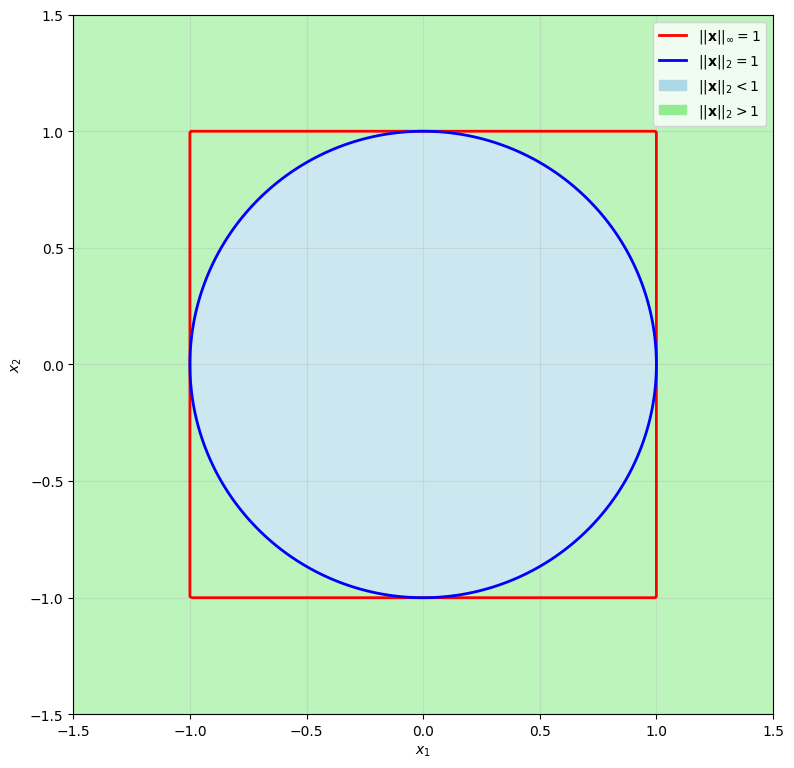
\includegraphics[width=0.8\textwidth]{4c.png}
\end{figure}

%%%%%%%%%%%%%%%%%%%%
\clearpage
\item[] \textbf{Question 5: Basic vector operations (20 points)} 
%%%%%%%%%%%%%%%%%%%%

Given two 3-dimensional vectors $\mathbf{a}, \mathbf{b}$, and three matrices $A \in \mathbb{R}^{2 \times 3}, B \in \mathbb{R}^{3 \times 2}, C \in \mathbb{R}^{2 \times 3}$, scalars $\beta_1, \beta_2$ with the values below:\\

\begin{gather*}
    \mathbf{a} = \begin{bmatrix} 1 \\ 3 \\ 5 \end{bmatrix} 
    \mathbf{b} = \begin{bmatrix} 2 \\ 4 \\ 6 \end{bmatrix} 
    \mathbf{A} = \begin{bmatrix} 1 & 2 & 3 \\ 2 & 4 & 6 \end{bmatrix} 
    \mathbf{B} = \begin{bmatrix} 7 & 8 \\ 9 & 10 \\ 11 & 12 \end{bmatrix} 
    \mathbf{C} = \begin{bmatrix} 1 & 0 & 0 \\ 0 & 0 & 1 \end{bmatrix} \\
    \mathbf{\beta_1} = 4, \mathbf{\beta_2} = 5
\end{gather*}



\begin{enumerate}
\item Compute the following operations by hand and show your work: (15 points)
\begin{enumerate}
    \item [(i)] Vector operations:
    $\mathbf{a} + \mathbf{b}, \quad \beta_1 \mathbf{a}, \quad \mathbf{a} \circ \mathbf{b}, \quad \beta_1 \mathbf{a} + \beta_2 \mathbf{b}$
    where $\circ$ denotes component-wise multiplication. (3 points)
    
    \item [(ii)] Matrix operations: $\beta_1 \mathbf{A}, \quad \mathbf{A} + \mathbf{B}, \quad \mathbf{A} + \mathbf{C}$. (3 points)
    
    \item [(iii)] Transpose operations: $(\mathbf{AB})^\top, \quad \mathbf{B}^\top \mathbf{A}^\top, \quad (\mathbf{A}^{\top})^{\top}, \quad (\mathbf{A} + \mathbf{C})^\top$. (3 points)
    
    \item [(iv)] Inner products and outer product: $\langle \mathbf{a}, \mathbf{b} \rangle, \quad \langle \mathbf{b}, \mathbf{a} \rangle, \quad \langle \mathbf{a}, \mathbf{a} \rangle, \quad \langle \mathbf{b}, \mathbf{b} \rangle, \quad \beta_1 \langle \mathbf{a}, \mathbf{b} \rangle, \quad \langle \beta_1 \mathbf{a}, \mathbf{b} \rangle, \quad \mathbf{b} \mathbf{a}^\top $. (3 points)
    
    \item [(v)] Determinants: $\det(\mathbf{AB}), \quad \det(\mathbf{BC})$. (3 points)
\end{enumerate}
\item Implement all the parts above using python (any programming language of your choice)  and show the answers and code. (5 points)
\end{enumerate}

\textbf{Solution:}

\begin{enumerate}
\item
\begin{enumerate}
\item [(i)] $\mathbf{a} + \mathbf{b} = \begin{bmatrix} 1 \\ 3 \\ 5 \end{bmatrix} + \begin{bmatrix} 2 \\ 4 \\ 6 \end{bmatrix} = \begin{bmatrix} 1 + 2 \\ 3 + 4 \\ 5 + 6 \end{bmatrix} = \begin{bmatrix} 3 \\ 7 \\ 11 \end{bmatrix}$\\
            $\beta_1 \mathbf{a} = 4 \begin{bmatrix} 1 \\ 3 \\ 5 \end{bmatrix} = \begin{bmatrix} 4 \cdot 1 \\ 4 \cdot 3 \\ 4 \cdot 5 \end{bmatrix} = \begin{bmatrix} 4 \\ 12 \\ 20 \end{bmatrix}$\\
            $\mathbf{a} \circ \mathbf{b} = \begin{bmatrix} 1 \\ 3 \\ 5 \end{bmatrix} \circ \begin{bmatrix} 2 \\ 4 \\ 6 \end{bmatrix} = \begin{bmatrix} 1 \cdot 2 \\ 3 \cdot 4 \\ 5 \cdot 6 \end{bmatrix} = \begin{bmatrix} 2 \\ 12 \\ 30 \end{bmatrix}$\\
            $\beta_1 \mathbf{a} + \beta_2 \mathbf{b} = 4 \begin{bmatrix} 1 \\ 3 \\ 5 \end{bmatrix} + 5 \begin{bmatrix} 2 \\ 4 \\ 6 \end{bmatrix} = \begin{bmatrix} 4 \cdot 1 + 5 \cdot 2 \\ 4 \cdot 3 + 5 \cdot 4 \\ 4 \cdot 5 + 5 \cdot 6 \end{bmatrix} = \begin{bmatrix} 4 + 10 \\ 12 + 20 \\ 20 + 30 \end{bmatrix} = \begin{bmatrix} 14 \\ 32 \\ 50 \end{bmatrix}$
\item [(ii)] $\beta_1 \mathbf{A} = 4 \begin{bmatrix} 1 & 2 & 3 \\ 2 & 4 & 6 \end{bmatrix} = \begin{bmatrix} 4 \cdot 1 & 4 \cdot 2 & 4 \cdot 3 \\ 4 \cdot 2 & 4 \cdot 4 & 4 \cdot 6 \end{bmatrix} = \begin{bmatrix} 4 & 8 & 12 \\ 8 & 16 & 24 \end{bmatrix}$\\
             $\mathbf{A} + \mathbf{B}$ DNE bc dimensions are incompatible \\
             $\mathbf{A} + \mathbf{C} = \begin{bmatrix} 1 & 2 & 3 \\ 2 & 4 & 6 \end{bmatrix} + \begin{bmatrix} 1 & 0 & 0 \\ 0 & 0 & 1 \end{bmatrix} = \begin{bmatrix} 1 + 1 & 2 + 0 & 3 + 0 \\ 2 + 0 & 4 + 0 & 6 + 1 \end{bmatrix} = \begin{bmatrix} 2 & 2 & 3 \\ 2 & 4 & 7 \end{bmatrix}$
\item [(iii)] $(\mathbf{A}\mathbf{B})^\top = \left(\begin{bmatrix} 1 & 2 & 3 \\ 2 & 4 & 6 \end{bmatrix} \begin{bmatrix} 7 & 8 \\ 9 & 10 \\ 11 & 12 \end{bmatrix}\right)^\top = \begin{bmatrix} 1 \cdot 7 + 2 \cdot 9 + 3 \cdot 11 & 1 \cdot 8 + 2 \cdot 10 + 3 \cdot 12 \\ 2 \cdot 7 + 4 \cdot 9 + 6 \cdot 11 & 2 \cdot 8 + 4 \cdot 10 + 6 \cdot 12 \end{bmatrix}^\top = \\\begin{bmatrix} 58 & 64 \\ 116 & 128 \end{bmatrix}^\top = \begin{bmatrix} 58 & 116 \\ 64 & 128 \end{bmatrix}$\\
              $\mathbf{B}^\top \mathbf{A}^\top = \begin{bmatrix} 7 & 8 \\ 9 & 10 \\ 11 & 12 \end{bmatrix}^\top \begin{bmatrix} 1 & 2 & 3 \\ 2 & 4 & 6 \end{bmatrix}^\top = \begin{bmatrix} 7 & 9 & 11 \\ 8 & 10 & 12 \end{bmatrix} \begin{bmatrix} 1 & 2 \\ 2 & 4 \\ 3 & 6 \end{bmatrix} = \\\begin{bmatrix} 7 \cdot 1 + 9 \cdot 2 + 11 \cdot 3 & 7 \cdot 2 + 9 \cdot 4 + 11 \cdot 6 \\ 8 \cdot 1 + 10 \cdot 2 + 12 \cdot 3 & 8 \cdot 2 + 10 \cdot 4 + 12 \cdot 6 \end{bmatrix} = \begin{bmatrix} 58 & 116 \\ 64 & 128 \end{bmatrix}$\\
              $(\mathbf{A}^{\top})^{\top} = \left(\begin{bmatrix} 1 & 2 & 3 \\ 2 & 4 & 6 \end{bmatrix}^\top\right)^{\top} = \begin{bmatrix} 1 & 2 \\ 2 & 4 \\ 3 & 6 \end{bmatrix}^\top = \begin{bmatrix} 1 & 2 & 3 \\ 2 & 4 & 6 \end{bmatrix}$\\
              $(\mathbf{A} + \mathbf{C})^\top = \left(\text{part (ii)}\right)^\top = \begin{bmatrix} 2 & 2 & 3 \\ 2 & 4 & 7 \end{bmatrix}^\top = \begin{bmatrix} 2 & 2 \\ 2 & 4 \\ 3 & 7 \end{bmatrix}$
\item [(iv)] $\langle\mathbf{a}, \mathbf{b}\rangle = \mathbf{a}^\top\mathbf{b} = \begin{bmatrix} 1 & 3 & 5 \end{bmatrix} \begin{bmatrix} 2 \\ 4 \\ 6 \end{bmatrix} = 1 \cdot 2 + 3 \cdot 4 + 5 \cdot 6 = 44$\\
             $\langle\mathbf{b}, \mathbf{a}\rangle = \mathbf{b}^\top\mathbf{a} = \begin{bmatrix} 2 & 4 & 6 \end{bmatrix} \begin{bmatrix} 1 \\ 3 \\ 5 \end{bmatrix} = 2 \cdot 1 + 4 \cdot 3 + 6 \cdot 5 = 44$\\
             $\langle\mathbf{a}, \mathbf{a}\rangle = \mathbf{a}^\top\mathbf{a} = \begin{bmatrix} 1 & 3 & 5 \end{bmatrix} \begin{bmatrix} 1 \\ 3 \\ 5 \end{bmatrix} = 1 \cdot 1 + 3 \cdot 3 + 5 \cdot 5 = 35$\\
             $\langle\mathbf{b}, \mathbf{b}\rangle = \mathbf{b}^\top\mathbf{b} = \begin{bmatrix} 2 & 4 & 6 \end{bmatrix} \begin{bmatrix} 2 \\ 4 \\ 6 \end{bmatrix} = 2 \cdot 2 + 4 \cdot 4 + 6 \cdot 6 = 56$\\
             $\beta_1 \langle\mathbf{a}, \mathbf{b}\rangle = 4 \cdot 44 = 176$\\
             $\langle \beta_1 \mathbf{a}, \mathbf{b} \rangle = (4\mathbf{a})^\top \mathbf{b} = \left(4 \begin{bmatrix} 1 \\ 3 \\ 5 \end{bmatrix}\right)^\top \begin{bmatrix} 4 & 12 & 20 \end{bmatrix} \begin{bmatrix} 2 \\ 4 \\ 6 \end{bmatrix} = 4 \cdot 2 + 12 \cdot 4 + 20 \cdot 6 = 176$\\
             $\mathbf{b} \mathbf{a}^\top = \begin{bmatrix} 2 \\ 4 \\ 6 \end{bmatrix} \begin{bmatrix} 1 & 3 & 5 \end{bmatrix} = \begin{bmatrix} 2 \cdot 1 & 2 \cdot 3 & 2 \cdot 5 \\ 4 \cdot 1 & 4 \cdot 3 & 4 \cdot 5 \\ 6 \cdot 1 & 6 \cdot 3 & 6 \cdot 5 \end{bmatrix} = \begin{bmatrix} 2 & 6 & 10 \\ 4 & 12 & 20 \\ 6 & 18 & 30 \end{bmatrix}$
\item [(v)] $\det(\mathbf{AB}) = \det\left(\begin{bmatrix} 1 & 2 & 3 \\ 2 & 4 & 6 \end{bmatrix} \begin{bmatrix} 7 & 8 \\ 9 & 10 \\ 11 & 12 \end{bmatrix}\right) = \det\left(\begin{bmatrix} 58 & 64 \\ 116 & 128 \end{bmatrix}\right) = 58 \cdot 128 - 64 \cdot 116 = 7424 - 7424 = 0$\\
             $\det(\mathbf{BC}) = \det\left(\begin{bmatrix} 7 & 8 \\ 9 & 10 \\ 11 & 12 \end{bmatrix} \begin{bmatrix} 1 & 0 & 0 \\ 0 & 0 & 1 \end{bmatrix}\right) = \det\left(\begin{bmatrix} 7 & 8 & 0 \\ 9 & 10 & 0 \\ 11 & 12 & 0 \end{bmatrix}\right) = 7 \det\left(\begin{bmatrix} 10 & 0 \\ 12 & 0 \end{bmatrix}\right) - 8 \det\left(\begin{bmatrix} 9 & 0 \\ 11 & 0 \end{bmatrix}\right) + 0 = 7(10 \cdot 0 - 0 \cdot 12) - 8(9 \cdot 0 - 0 \cdot 11) + 0 = 0 - 0 + 0 = 0$
\end{enumerate}
\item Code:
\begin{lstlisting}[language=python]
a = np.array([1, 3, 5])
b = np.array([2, 4, 6])
A = np.array([[1, 2, 3],
              [2, 4, 6]])
B = np.array([[7, 8],
              [9, 10],
              [11, 12]])
C = np.array([[1, 0, 0],
              [0, 0, 1]])
beta_1 = 4
beta_2 = 5
\end{lstlisting}
\begin{lstlisting}[language=python]
a + b
\end{lstlisting}
\begin{verbatim}
array([ 3,  7, 11])
\end{verbatim}
\begin{lstlisting}[language=python]
beta_1 * a
\end{lstlisting}
\begin{verbatim}
array([ 4, 12, 20])
\end{verbatim}
\begin{lstlisting}[language=python]
a * b
\end{lstlisting}
\begin{verbatim}
array([ 2, 12, 30])
\end{verbatim}
\begin{lstlisting}[language=python]
beta_1 * a + beta_2 * b
\end{lstlisting}
\begin{verbatim}
array([14, 32, 50])
\end{verbatim}
\begin{lstlisting}[language=python]
beta_1 * A
\end{lstlisting}
\begin{verbatim}
array([[ 4,  8, 12],
       [ 8, 16, 24]])
\end{verbatim}
\begin{lstlisting}[language=python]
A + B
\end{lstlisting}
Successful indication of DNE:
\begin{verbatim}
ValueError: operands could not be broadcast together with shapes (2,3) (3,2)
\end{verbatim}
\begin{lstlisting}[language=python]
A + C
\end{lstlisting}
\begin{verbatim}
array([[2, 2, 3],
       [2, 4, 7]])
\end{verbatim}
\begin{lstlisting}[language=python]
(A @ B).T
\end{lstlisting}
\begin{verbatim}
array([[ 58, 116],  
       [ 64, 128]])
\end{verbatim}
\begin{lstlisting}[language=python]
B.T @ A.T
\end{lstlisting}
\begin{verbatim}
array([[ 58, 116],
       [ 64, 128]])
\end{verbatim}
\begin{lstlisting}[language=python]
(A.T).T
\end{lstlisting}
\begin{verbatim}
array([[1, 2, 3],
       [2, 4, 6]])
\end{verbatim}
\begin{lstlisting}[language=python]
(A + C).T
\end{lstlisting}
\begin{verbatim}
array([[2, 2],
       [2, 4],
       [3, 7]])
\end{verbatim}
\begin{lstlisting}[language=python]
    np.inner(a, b)
\end{lstlisting}
\begin{verbatim}
np.int64(44)
\end{verbatim}
\begin{lstlisting}[language=python]
    np.inner(b, a)
\end{lstlisting}
\begin{verbatim}
np.int64(44)
\end{verbatim}
\begin{lstlisting}[language=python]
    np.inner(a, a)
\end{lstlisting}
\begin{verbatim}
np.int64(35)
\end{verbatim}
\begin{lstlisting}[language=python]
    np.inner(5, 6)
\end{lstlisting}
\begin{verbatim}
np.int64(176)
\end{verbatim}
\begin{lstlisting}[language=python]
    beta_1 * np.inner(a, b)
\end{lstlisting}
\begin{verbatim}
np.int64(176)
\end{verbatim}
\begin{lstlisting}[language=python]
    np.inner(beta_1 * a, b)
\end{lstlisting}
\begin{verbatim}
np.int64(176)
\end{verbatim}
\begin{lstlisting}[language=python]
    np.outer(b, a)
\end{lstlisting}
\begin{verbatim}
array([[ 2,  6, 10],
       [ 4, 12, 20],
       [ 6, 18, 30]])
\end{verbatim}
\begin{lstlisting}[language=python]
np.linalg.det(A @ B)
\end{lstlisting}
\begin{verbatim}
np.float64(0.0)
\end{verbatim}
\begin{lstlisting}[language=python]
np.linalg.det(B @ C)
\end{lstlisting}
\begin{verbatim}
np.float64(0.0)
\end{verbatim}
\end{enumerate}
\end{enumerate}
\end{document}

